\chapter{Experiments}
\label{chap:experiments}
When evaluating the research question of this thesis,
we started by assessing Human performance on the task.

We then moved onto \ac{ml} models. 
First, we created a \ac{mlr} to set up
a baseline for the more complex models and to check,
whether certain tasks are not too trivial for \ac{ml} models,
due to a problems in the dataset.

We followed with transformer models. We decided
to fine-tune, rather than train from scratch. While
we had plenty of data, we assumed that the pre-trained
models would contain intrinsic language knowledge,
which could be helpful for the tasks.

This decision meant that we couldn't modify
the architecture of the models. To create the
best models, we could only change the training setting
and backbones themselves.

This chapter will describe the transformer experiments
as well as both baseline and human ones.

\section{Human performance}
\label{sec:human}
To evaluate human performance, we let four evaluators classify the articles on 
the Test Human set (see \autoref{sec:splits}).
Each evaluator got access to Google Sheet\footnote{https://docs.google.com/},
where they had to assign each document a correct label for each task.
Evaluators were offered all options for each task, not just the subset from Test Human set.
We will denote averaged scores of all evaluators as \textbf{Human}.

\section{Baseline}
For a baseline, we have used \ac{mlr} with TF-IDF features.
TF-IDF features setting used:
\begin{enumerate}
    \item Tokenization method: lowercased text with MosesTokenizer\footnote{\url{https://pypi.org/project/mosestokenizer/}}.
    \item Maximum document frequency: 1\%
    \item Ngrams: 1-2
    \item Minimum document frequency: 90 documents
    \item Stop words: Czech stop words from stop-words package\footnote{\url{https://pypi.org/project/stop-words/}}.
\end{enumerate}
Similar to \textcite{strakaSumeCzechLargeCzech2018a}, we have added the following additional features:
\begin{enumerate}
    \item Number of words
    \item Number of words with only non-alphabetic characters
    \item Number of uppercase words
    \item Number of digits words
    \item Number of capitalized words
\end{enumerate}
We run a grid search over the following hyperparameters:
\begin{enumerate}
    \item Inverse Regularization term: $1, 10, 100, 1000$
\end{enumerate}
We selected the best model based on the F1 Macro score on the validation set.
As for the solver, we have used SAGA~\parencite{defazioSAGAFastIncremental2014}
implementation from Scikit-learn library\footnote{\url{https://scikit-learn.org}},
with max iterations set to 800 and an early stopping tolerance of 0.001.
With this setting, we created 2 models; \textbf{LR-50} with 50k TF-IDF features
and \textbf{LR-200} with 200k TF-IDF features.

\section{Backbone models}
\label{sec:backbone}
For backbone models, we have used \textbf{RobeCzech}, \textbf{Fernet-News},
and \textbf{GPT-3}. We chose RobeCzech and Fernet-News as both are Czech mono-lingual transformers
with the same architecture and the relatively same number of parameters~(see \autoref{tab:czech-monolingual}).
The main difference is the training data and training setting~(see \autoref{sec:robe-czech}, \autoref{sec:fernet}). We chose the
GPT-3, as we were interested in its multi-lingual capabilities.

\subsection{RobeCzech and Fernet-News}
\label{sec:base-models}

\begin{figure}[h]
    \centering
    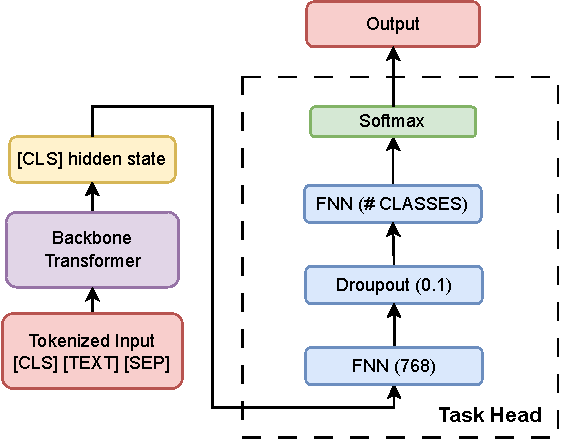
\includegraphics[width=0.7\linewidth]{img/transformer/fine_tune.pdf}
    \caption{Fine-tuning architecture for the classification task.}
    \label{fig:class-tune}
\end{figure}

For fine-tuning, we mostly followed hyperparameter settings
recommend by \textcite{sunHowFineTuneBERT2020}.
As for architecture, we took the backbone model and replaced
the head as shown in~\autoref{fig:class-tune}.
We have used the following hyperparameters:
\begin{enumerate}
    \item Effective Batch size
    \footnote{By effective batch size, we mean:  
    $\textrm{gradient accumulation steps} \cdot \textrm{number of devices}
    \cdot \textrm{batch size}$
    }: 48
    \item Number of epochs: 2
    \item Sequence length: maximum 512 tokens with dynamic padding per batch
    \item Weight decay: 0
    \item Optimizer: AdamW with epsilon 1e-8, beta1 0.9, beta2 0.999.
    \item Scheduler: Linear warmup with 0.1 warmup ratio
    \item Unfrozen layers: 12
    \item Truncation: First 512 tokens
    \item Unfrozen Embeddings: False
\end{enumerate}
To find the best \ac{lr}, we run a grid search for each model and task.
However, we quickly found out that the Fernet-News was more sensitive to the high \ac{lr}
and thus, we couldn't apply the same \acp{lr} for both models.
We have used the following \acp{lr}:
\begin{enumerate}
    \item RobeCzech: 3e-5, 4.5e-5, 7.5e-5
    \item Fernet-News: 1e-5, 2e-5, 3e-5
\end{enumerate}
Grid search only run for 0.4 portion of the first epoch and \ac{lr} with the best validation 
F1 macro score was selected.
For implementation, we have used \textit{Pytorch Lightning 2.0}\footnote{\url{https://www.pytorchlightning.ai/}},
\textit{\ac{hf} Transformers 4.24}\footnote{\url{https://huggingface.co/docs/transformers/index}}
and \textit{Pytorch 2.0.0}\footnote{\url{https://pytorch.org/}}.
We trained models on \ac{aic} with a single GeForce RTX 2080 Ti.
We denote the models as \textbf{R-Base} and \textbf{F-Base}.

\subsection{GPT-3}
\label{sec:gpt-3}
We have chosen Ada version of GPT-3, as it is the cheapest.
Ada costs 0.00004\$/1k tokens for fine-tuning and 0.00016\$/1k tokens for a inference.
As the model architecture is not adjustable, the fine-tuning works
as text generation fine-tuning.
Thus we only provide query (Text of article) and text completion (Class).
To save the cost, we fine-tuned it in a multi-task setting.
Thus for every task, we created a label in the format: \textit{Full Server Name} \textit{Category} \textit{Gender} \textit{Day of week}.
We used Czech translations for task classes, as we assumed that it would be easier for the model to learn,
since the content is in Czech.

The Ada model takes a maximum of 2048 tokens; thus, we truncated documents to 1400 characters.
To save the costs, we used \textbf{Train-small} (see \autoref{sec:splits}) for fine-tuning and
\textbf{Test-small} (see \autoref{sec:splits}) for inference.
We then finetuned for 2 epochs.

We also fine-tuned and evaluated RobeCzech and Fernet-News on the same datasets for comparison.
We denote the models as \textbf{GPT-3}, \textbf{R-Small} and \textbf{F-Small}.

\section{Fine-tuning}
\label{sec:finetuning}
We were interested in ways to improve fine-tuning performance without changing the backbone model.
We tried three approaches inspired by \textcite{howardUniversalLanguageModel2018a} and \textcite{sunHowFineTuneBERT2020}.
All the experiments were done on \textbf{RobeCzech} model, with settings as in \autoref{sec:robe-czech}
unless stated otherwise.

\subsection{Truncation}
\label{sec:truncation}
The base models are trained with truncation to the first 512 tokens.
Due to the nature of the task,
we hypothesized that the last part might contain more relevant information:
\begin{quote}
    Pro Idnes.cz Jana Křížová
\end{quote}
Therefore, we tried to truncate the text by taking the last 512 tokens.
We denote the model as \textbf{Truncate}.

\subsection{\acl{flm}}
\label{sec:task-modeling}
Both \textcite{howardUniversalLanguageModel2018a} and \textcite{sunHowFineTuneBERT2020}
found that \acf{flm} on task dataset can improve performance.
We used the same approach.
For Lanuage Modelling we have used the following hyperparameters:
\begin{enumerate}
    \item Effective Batch size: 198
    \item Number of epochs: 10
    \item Sequence length: 512 tokens
    \item Sequence sampling: Cross document
    \item Masking: 15\% token change (80\% random, 10\% replace, 10\% keep)
    \item Optimizer: AdamW with epsilon 1e-8, beta1 0.9, beta2 0.98
    \item Unfrozen Embeddings: True
\end{enumerate} 
We have then used the trained model as the backbone
and trained with the same setting as the Base model.
We denote the resulting model as \textbf{LM-Tune}


\subsection{Gradual unfreezing with discriminative learning rates}
\label{sec:gradual-unfreezing}
\textcite{howardUniversalLanguageModel2018a} showed that we could improve model performance by gradually unfreezing layers
. We know the method was 
used with RNNs, and the results might not be directly comparable, but we wanted to try it anyway.
We have also add a discriminative learning rate which sets samller \acp{lr} for the lower layers.
We set the discriminative factor to 0.95 as in \parencite{sunHowFineTuneBERT2020}.
The \ac{gu} is not well described in \parencite{howardUniversalLanguageModel2018a}, thus we tried two approaches:
\begin{enumerate}
    \item \textbf{Grad-12} Unfreeze 1 layer per epoch, starting from the last layer, and run for 12 epochs.
    \item \textbf{Grad-24} Unfreeze 1 layer per epoch,
    starting from the last layer, and run for 24 epochs~(12 epochs in the full unfrozen state).
\end{enumerate}
The epoch lengths are adjusted, so that the total number of optimizer steps stays the same as in \autoref{sec:base-models}~(full 2 epochs).
For both approaches, we unfreeze the classifier layer at epoch 0 with \ac{lr} decaying from $1e-3$ to $ 5e-5$.
The first unfrozen layer has \ac{lr} peak at best \ac{lr} found at \autoref{sec:robe-czech} for a given task.
The remaining layers are adjusted based on the discriminative learning rate.
Each unfrozen layer has a scheduler with the same setting as base model tuning~(\autoref{sec:backbone}).
 However, it starts scheduling when the layer is unfrozen.
The remaining setting stays the same as in base model tuning~(\autoref{sec:backbone}).

\section{Final Model}
\label{sec:final-model}
Finally, we created a model combining the best backbone and fine-tuning approaches.
Therefore, we used \textbf{RobeCzech} as a backbone with \ac{flm}.
Additionaly we reused the classifier scheduling as in \autoref{sec:gradual-unfreezing}.
Due to the results of \textit{Short} models, we also set the warmup steps to just 0.01 and added
Most-recent sampling.
\subsection{Most-recent sampling}
To add weight to more recent articles, we sample article $i$ the dataset with the following probability:
\begin{equation}
    P(i) = \frac{\exp(2 d_i)}{\sum_{j=1}^{n} \exp(2 d_j)}
\end{equation}
where $d_i$
\begin{equation}
    d_i = \frac{t_i}{\max_{0\le j \le n}{t_j}}
\end{equation}
where $t_i$ is the time difference between the published date of article $i$ and the dataset's eldest article in days.
